\documentclass[conference]{IEEEtran}
\usepackage{array}
\usepackage{url}
\usepackage{graphics}
\usepackage{graphicx}
\usepackage{url}
\usepackage{float}
\usepackage{tabularx}
\usepackage{multirow}
\usepackage{listings}
\usepackage{color}
\usepackage{xspace}
\usepackage{paralist}
%\usepackage{xcolor}
%\usepackage{sloppy}
\usepackage{array}
%\usepackage{cite}
\usepackage{fixltx2e}
\usepackage{soul}
\usepackage{amsmath}
\usepackage{caption}
\begin{document}
%
% paper title
% Titles are generally capitalized except for words such as a, an, and, as,
% at, but, by, for, in, nor, of, on, or, the, to and up, which are usually
% not capitalized unless they are the first or last word of the title.
% Linebreaks \\ can be used within to get better formatting as desired.
% Do not put math or special symbols in the title.

\title{Hacking at the divide between polar science and HPC: Using hackathons as training tools}

\author{\IEEEauthorblockN{Jane Wyngaard\IEEEauthorrefmark{1},
Heather Lynch\IEEEauthorrefmark{2},
Jaroslaw Nabrzyski\IEEEauthorrefmark{1},
Allen Pope\IEEEauthorrefmark{3} and
Shantenu Jha\IEEEauthorrefmark{4}}

\IEEEauthorblockA{\IEEEauthorrefmark{1}Center for Research Computing,
University of Notre Dame,
South Bend, IN \\ 
Email: jwyngaar@nd.edu, naber@nd.edu}
\IEEEauthorblockA{\IEEEauthorrefmark{2}Ecology \& Evolution, Institute for Advanced Computational Sciences\\
Stony Brook University,
Stony Brook, NY,
Email: heather.lynch@stonybrook.edu}
\IEEEauthorblockA{\IEEEauthorrefmark{3}National Snow \& Ice Data Center,
CIRES, University of Colorado Boulder,
Boulder, CO\\ 
Email:allen.pope@nsidc.org}
\IEEEauthorblockA{\IEEEauthorrefmark{4}Department of Computer Engineering,
Rutgers University \\
New Brunswick, NJ,
Email:shantenu.jha@rutgers.edu}
}

\maketitle

\begin{abstract}
Given the current scientific questions of societal significance, such as those related to climate change, there is an urgent need to equip the scientific community with the means to effectively use high-performance and distributed computing (HPDC), Big Data, and tools necessary for reproducible science.  The {\it Polar Computing RCN} project (\url{http://polar-computing.org}) is a National Science Foundation funded Research Coordination Network, which has been tasked with bridging the current gap between the polar science and HPDC communities. In this paper we discuss the effectiveness of ``hackathons'' as a model for implementing both the pedagogical training and the hands-on experience required for HPDC fluency.  We find hackathons effective in: (i) Conveying to a science user how and why HPDC resources might be of value to their work, (ii) Providing a venue for cross discipline vocabulary exchange between domain science and HPDC experts, (iii) Equipping science users with customized training that focuses on the practical use of HPDC for their applications, (iv) Providing hands-on training with a realistic domain-specific application in a community of one's peers, but are (v) an incomplete training model that requires supplementation via domain science specific HPDC training materials. In addition to their pedagogical benefits, hackathons provide additional benefits in terms of team building, networking, and the creation of immediately usable products that can speed workflows both for those involved in the hackathon as well as others not involved in the hackathon itself. 
\end{abstract}


\section{Introduction}
% no \IEEEPARstart
Climate change in the 20th and 21st century is one of the most pressing issues of our day, and the inherently global scale of the problem creates demand for HPDC resources. No where is climate change more dramatic than in the polar regions~\cite{Nelson2007}. Recent studies indicate accelerated thawing of permafrost, receding Arctic sea ice, and accelerating mass loss from the Greenland and Antarctic ice sheets, and smaller ice cap and mountain glaciers. Understanding the changing polar regions and connections to global climate involves working with multiple heterogeneous sets of data (in multiple formats and ranging spatial and temporal resolutions), from multiple distinct domains of expertise. Oceanography, Climatology, Glaciology, Meteorology, and Biology (along with the many subfields within each) all generate and use their own data sets, which may include field measurements, high-resolution observations from satellites, airborne imagery, and computer model outputs. Computational approaches now support faster and more fine-grained integration and analysis of these and other data types, and provide a better understanding of the complex processes that are rapidly changing our climate.  

However, despite these data- and compute-intensive scientific needs, polar science (along with other disciplines) is poorly represented in the use of HPDC resources. Through informal community engagement, a Polar-HPDC workshop in 2014~\cite{Workshop2014}, and the 2016 hackathon reported on here, we have identified two primary reasons for this gap: (1) a lack of community awareness of available compute resources, and (2) a lack of appropriate training for scientists interested in using HPDC for science applications. 

There is therefore an urgent need to equip the scientific community to use high-performance and distributed computing (HPDC) and Big Data technologies\footnote{ We use the overused term 'Big Data' and Big Data technologies to represent scalable methods and technologies to address any of the 'V's'  -- volume, velocity, variety and veracity -- noting that 'big' is relative to historic norms and varies tremendously across domains.}. The scientific questions facing society increasingly require not only greater computing power but also tools for sharing code and data that minimize duplication of effort and allow for reproducible science. Fortunately, for many applications, the technology for such already exists. Unfortunately, there is a gap in skill set and tool usability that needs to be overcome on a broad scale in order for these methods and tools to be used efficiently and effectively by science domain experts. While rapid development in the field of HPDC has eliminated many of the technical barriers to solving modern scientific problems, the pace of change has made it more difficult than ever for domain scientists to keep pace. Accordingly, we need a renewed focus on training domain scientists to use HPDC resources, methods, and tools effectively. 

The above challenges and the resulting gap have now been formally recognized
by funding agencies and researchers, not just in the polar sciences. This has
led to experiments with new pedagogical approaches. We propose here an
alternative HPDC education approach tailored to equipping domain expert
scientists who are traditionally not users of HPDC.  We refer to this as
ALITE-HPDC education. ALITE-HPDC training is focused on communicating what's
Appropriate \& Available (A), communicating clearly the Lingo (L) of HPDC, is
Tailored (T) to only cover those aspects of HPDC that are essential for a
domain's users, and is Extensible (E) and modular.  

The ALITE training model for HPDC is similar to agile development in software;
progressively growing yet functionally useful at every stage. This is in
contrast to the waterfall method where step changes in (learnt) capabilities
are realized. Even though the ALITE training model has a different scope and
purpose  compared to traditional frameworks for categorizing educational goals
such as Bloom's Taxonomy~\cite{bloom}, we believe the ALITE maps well to the
the "Knowledge" and "Comprehension" tiers of 
Blooms Taxonomy~\cite{bloom-vanderbilt}.

Taking a lesson from the long running and widely successful introduction to scientific computing offered by Software Carpentry (SWC)~\cite{Wilson2014-pc}, we believe there should be training materials focused on only those components of HPDC that are absolutely ``need to know'' for our audience. This approach recognizes that domain scientists using HPDC may lack the time or ``mental bandwidth'' to learn any details irrelevant to running their compute jobs. The three stages of our ALITE-HPDC training program focus on creating a scientific community that is HPDC-aware, HPDC-literate, and HPDC-trained, respectively, at the expense of more in depth training in hardware and algorithms typical of current HPDC education.  Researchers who are able to use HPDC resources successfully, even at a basic level, will feel empowered and motivated to learn more, and this can most easily be done if the initial time requirement for getting started is minimized. If, at a later stage, greater in-depth knowledge is required for code optimization, HPDC-engaged researchers will be equipped to seek out and gain from further training, such as is already widely available through the existing documentation for HPDC resources.


We need to target both graduate students and established researchers, given that HPDC resources and the reasons for their need are a recent development in many domains. Effective mid-career training is particularly difficult to achieve as it is difficult for PIs to carve out enough time for learning new skills. To address this challenge, lessons need to be broken up into deliberately small chunks and formatted such that they can be completed in the margins of other commitments. By focusing only on those skills that are ``need to know'', and by re-packaging that information in small chunks, we believe it possible to overcome some of these hurdles.  In the polar community specifically, it is often easiest to carve out time for such training when researchers are in the field, since polar deployments can involve long periods of uninterrupted ``downtime''.  This means, however, that these researchers are also often working with limited to zero connectivity, a factor which must therefore be considered when designing training materials. Further, even for non-field researchers or those without significant downtime, breaking training into smaller, independent chunks will facilitate uptake across the community.

Recognizing the importance of this knowledge gap, and particularly in the polar sciences, the National Science Foundation has funded a number of initiatives tasked with addressing this issue.  Amongst them is the Research Coordination Network (RCN) that the authors lead. The remainder of this paper follows with: Section II describes the reasons behind the described gap's persistence, Section III reviews some of the novel approaches being undertaken to address these such as short intense courses and hackathons, Section IV describes our use of a hackathon-based model, and finally Section V presents our conclusions.

\section{Challenges perpetuating the divide}
As discussed, through surveys and community workshops we have identified two primary reasons for the relatively low uptake of HPDC by the polar community.  

\begin{enumerate}[\setlength{\listparindent}{\parindent}]
\item \textit{Polar science professionals are (in general) poorly equipped to use HPDC resources:
We attribute this to five causes.}
\begin{enumerate}[\setlength{\listparindent}{\parindent}]
\item \textbf{Rate of technological change:} Priority in training scientists is unavoidably given to the domain science itself. Yet, the rate of technological change means easy-to-use tools of abstraction and formal undergraduate and graduate HPDC training generally lags far behind. 
\item \textbf{Momentum: } In our experience senior researchers are sometimes the slowest to adopt new technologies in their own workflows, which makes their adoption into formal coursework slow. They are also unable to train graduate students in these skills and may discourage students from using workflows that ``break with tradition'' in terms of curent lab methodologies.
\item \textbf{Limited Time: }The time available for established researchers to become HPDC proficient is extremely limited, an issue that is exacerbated in the polar community for researchers that spend considerable amounts of time in remote field camps. For this subset of the community, training and analyses have to be completed in the relatively small window between the conclusion of one field season and the start of planning for the next. 
\item \textbf{Inappropriate material: }Most HPDC resources have detailed documentation, often accompanied by optional training manuals and courses (both in face to face formats and offered as remote or recorded materials). However, these materials generally assume a relatively high level of programming, computer sophistication, and understanding of terminology that is often inappropriate for a general science audience.  

The materials' inaccessibility is in part due to a missing common vocabulary. In order for engineers and computer scientists to work with science users on applying HPDC resources to science challenges, a degree of common vocabulary is necessary. While HPDC terminology can be taught to all users, interpreting each science domain's terminology into common language requires partnership and direct engagement. Even a small number of HPDC-fluent scientists in each domain can have an enormously positive impact on their local communities, because they can explain terms and procedures in a way that is tangible to the community, and can address language or software specific questions.

Training materials also often prematurely focus on the details of the hardware, and fail to communicate why these details are of relevance. Emphasis should instead be given to running any job successfully, with details on computing efficiency coming only after a user is comfortable with the system and motivated to delve deeper. 

Finally, due to the focus on hardware and optimization, the materials are forced to gloss over the practical elements of job submission (ignoring the possible hurdle of even using a terminal interface first), to focus on theoretical elements aimed at current users interested in optimizing their code or gaining greater efficiency. 

\item \textbf{Limited HPDC support staff on campuses: } As noted above, advanced HPDC ecosystems are continuously improving but therefore also changing. Support staff for advanced HPDC has proven to be a critical consideration for campuses which is often lacking both in presence, and when present in allocation of time to training HPDC-beginners. The NSF has recognized this problem and is seeking to rectify it.  One such program is ``The advanced cyberinfrastructure research and education facilitators virtual residency: Toward a national cyberinfrastructure workforce''~\cite{Neeman2016-uz}.
\end{enumerate}

In addition to the systemic factors above, there are also many further obstacles which contribute to making available training materials often inaccessible for polar scientists. For instance, relatively simple things, like command line scripting, can be a major barrier for new HPDC users that lack a formal computer science background. Similarly, requesting time on HPDC resources often requires users to answer questions that they are ill prepared to answer, such as: ``How many nodes do you need?'', or ``How many compute units are requested?''.  

In other words, whereas HPDC appears at the end of a comprehensive program in a traditional computer science curriculum, domain scientists are looking to use HPDC resources with relatively little programming experience outside of the specific language or program they may be using for their research. If learning HPDC takes too long, scientists under tight research deadlines are likely to fall back on highly inefficient local compute solutions (their laptop, for example). Therefore, there is a great need for HPDC training materials that are stripped down to only those elements that are ``need to know'' for a first time user of a specific domain. These initial elements are focused on the practice of HPDC with a bare minimum of HPDC theory or the specific hardware of the system they are using.
\item \textit{A lack of knowledge of what resources are available:}
In many cases HPDC resources (including: hardware, software, and human support) exist specifically to serve the domain sciences, and yet some specializations may have little to no knowledge of what is available. 

Project such as US NSF funded XSEDE\footnote{"Extreme Science and Engineering Discovery Environment (XSEDE), is the most advanced, powerful, and robust collection of integrated advanced digital resources and services in the world. It is a single virtual system that scientists can use to interactively share computing resources, data, and expertise." www.xsede.org} \cite{noauthor_undated-lh}, are working to overcome this gap using such mechanisms as Campus Champions.  Given this, we believe that after solving the training problem, researchers will be equipped to find the resources they need. \end{enumerate} We believe a focus on the ALITE-education elements will address many of the pedagogical issues discussed.  And that this training should go beyond theory to incorporate relevant hands-on experience using HPDC resources.

\section{Related Work}
The NSF has long funded broad work in graduate training for interdisciplinary expertise via, among other mechanisms, the Integrative Graduate Education and Research Trainee-ship program \cite{noauthor_undated-bu}.  This program ran from 1997-2013 and has more recently been succeeded by the NSF Research Training program [NRT]~\cite{NRT}.  Both aim to develop institutional level multidisciplinary training tracks across all the sciences. These have been judged successful as far as their high level goals of creating ``more interdisciplinary educational experiences'', equipping students with ``the professional skills relevant to working in the 21st century'' and preparing students for ``a wide range of careers''\cite{National2006}. However, these programs do not specifically call out the need for smaller scale interdisciplinary training as discussed here.  Nor do they extend to early- and mid-career scientists looking to learn new skills. Within the NRT program, there is also currently no project specifically targeting the interdisciplinary needs of polar sciences.

Looking at HPDC training programs specifically, Louisiana State University developed ``A practical and comprehensive graduate course preparing students for research involving scientific computing''~\cite{Allen2011-qx}. The curriculum covers a range of topics appropriate to an introductory level course, including SSH, OpenGL, version control, networks and data, simulations and application frameworks, scientific visualization, and distributed scientific computing. Alternatively, the University of Oklahoma  developed ``Supercomputing in plain English''~\cite{Neeman2002-dk} that has been used for many years by Oklahoma and other institutes~\cite{Neeman2008-mj}.  Their curriculum includes the even more advanced topics of: shared memory, multi-threading, multicores, storage hierarchies, Instruction Level Parallelism, and compiler optimizations.  Finally, XSEDE itself offers both off-line and online training focused on systems and software supported by their service providers. Topics offered include: ``high performance computing, visualization, data management, distributed and grid computing, science gateways, and more.''~\cite{noauthor_undated-ht}.  

In the Louisiana State University course reported on in~\cite{Allen2011-qx}, attendees were largely drawn from computer science, systems science, or civil engineering graduates, yet it was found that even these domains required additional preparatory training. ``Supercomputing in plain English'', on the other hand, was targeted at non-programmers, but organizers still found that a 1 hr weekly expert follow-up with attendees was also necessary for up to two years following the course.  Finally, a review of the XSEDE training materials also reveals that it also assumes a base level of Computer Science knowledge that is unreasonable to expect of most polar scientists.

These lists of curricula topics offers a view into the complexity and depth that is considered necessary in an introductory level course to HPDC. Yet the implementation and real world experiences of teaching these courses confirms that traditional HPDC training materials are largely inaccessible to non-programmers. A counterexample to this common problem is provided by The Software Carpentry Foundation, which has been a dominant and successful pioneer of scientific programming training for people with non-computer science backgrounds. Over the past 2 decades SWC has ``evolved from a week-long training course at the US national laboratories into a worldwide volunteer effort to raise standards in scientific computing''~\cite{Wilson2014-pc}. They have found that an investment of 25 hours of lectures, plus practical work, can improve productivity of non-CS graduate students by 20\%~\cite{Wilson_undated-yk}. Further, they report 80-90\% of attendees are glad they attended and would recommend it to others. In 2013 alone, their materials were used to train 4300 scientists~\cite{Wilson2014-pc}.

Software Carpentry, and its sibling Data Carpentry~\cite{Mimno2016-cw} - which focuses more on skills for analysis than programming - have used their extensive experience to refine the model into its current format: 2 days, host driven, face-to-face, essentials-only, practical, and feedback intensive. To enable use-scalability and efficient community updating and improvement, all materials are published under a Creative Commons license on Github. Their course content, however, does not currently include HPDC specific topics, although the concept of a 'HPC Carpentry' has been raised many times within the community~\cite{Datacarpentry_undated-zl} and beyond~\cite{noauthor_undated-zw}, and is the subject of multiple discussion threads online. 

Believing it to be one of the several important components required to overcome the barriers between polar science and HPDC, we would like to see such a course developed in the near future. In its absence, however, as an RCN in 2016 we turned to another model of short and intense training, that of ``hackathons''. 

Originally the domain of Silicon Valley software companies, hackathons were used to collocate normally disparate team members for a period of intense coding. The concept, however, has since been eagerly adopted by a wide range of fields, such that it has now evolved to more often refer to collocating a group of diversely skilled people (coders, designers, artists, scientists, and many other professions), for a similar short intense period of work.  

Events are generally themed and focused on a given tool, challenge, or technology. Examples include the commercial and academic sectors engaging with each other and other professional communities outside their normal sphere such as: Barclays' competitive Financial Hackathon~\cite{noauthor_undated-rc} that sought innovative technology based financial products, or the annual non-competitive MIT Grand Hack~\cite{noauthor_undated-zx} that tackles health care challenges, or NASA engaging anyone who is interested in their annual Space apps challenge~\cite{noauthor_undated-rb}.  Alternatively, concerned citizens and bodies have run hackathons focused on specific social issues~\cite{noauthor_undated-qo,noauthor_undated-vs}, while the maker/hacker-space community use hackathons for everything from introducing K-12 children to basic electronics~\cite{Aboab2016-tk}, through to the Science Hack Day~\cite{noauthor_undated-qs} events which bring professional scientists and any other interested parties together to hack science problems.  Many other examples exist, of groups using the hackathon model to target different demographics, and cover all age groups.  

While hackathons were initially envisioned to produce innovation and productivity, a prominent and often noted by-product is the unique cross domain exchanging of skills and networking that can happen at such events. Students attending Major League Hacking~\cite{noauthor_undated-tz} (a competitive programming hackathon league for university students) for example, equate going to events with going to the gym for a skill set workout~\cite{Leckart2015-go}.  Alternatively,~\cite{Aboab2016-tk} advocates for the model to be formally recognized as a practical means of supporting cross disciplinary collaboration in academia. Supporting this perspective, post-event surveys from participants at DataViz~\cite{mattmann2015} (a 2014 polar datathon) rated the trans-disciplinary networking opportunity as the best part of the event.

\section{Our Experience with using a hackathon}
Given our task and the challenges reviewed, as a first step in exploring solutions and gaging community response, we hosted a hackathon in July 2016 co-located with the XSEDE annual meeting in Miami, Florida. The experience taught us that the hackathon model is an effective but imperfect and incomplete means of bridging the divide between HPDC and non-programmer domain specialist users (in this case in the polar sciences).  Specifically, as is elaborated on later, dedicated training input is still required, but we see the hackathon model as a valuable means of facilitating a path from taught theory to an accessible and applicable tool of relevance to specific users work. This section discusses the event, its successes, challenges, and the lessons learned.

\subsection{Preparation}
The RCN began by advertising a call for polar science proposals for a two day hackathon that would help the proposer use HPDC resource.  Suggested example project domains included: running slow code on faster hardware or using parallelization techniques, visualizing large data set, and exploring statistical computing and data manipulation centric problems.  In post event reviews, however, it was made clear to us that this was insufficient. That is, the ``what'' and ``how'' of HPDC technologies being of use to domain scientists needs to be better conveyed than just listing the above possibilities.  Domain relevant specific example case studies at least, should have instead been given.

This advertisement was circulated to multiple organizational list including: APECS, NSIDC, Cryolist, ESIP, INSTAAR, and the RCN steering committee members.  Additionally, eight key polar community members were requested to distribute the advert to their networks, and the RCN's own members' networks, twitter account, and website were used.

We debated amongst ourselves whether or not to request proposals publicly (perhaps as Github issues as other hackathons have done, or a public Google word document), or privately.  In the end we requested they be private, using EasyChair.  In retrospect and based on attendee responses this was the correct decision for this community, as there is a valid fear of being ``scooped'' scientifically.  We also believe personal emails to relevant professors would likely see more early career polar scientists hearing about the RCN activities and perhaps go someway to allaying fears.


In response to our advertisements we received seven proposals approximately two months prior to the event. Notably, three of these concerned a common challenge, performing segmentation and classification processing on remotely sensed sea ice imagery. Given the processing burden this analysis can incur it was determined that there is a real community need for a set of open source and accessible image processing tools to carry out such in a scalable manner on HPDC resources.  These three teams were therefore invited to join a single team tasked with tackling this jointly.  

Of the remaining four additional submissions, one was judged to be highly appropriate but indicated that the proposer already had access to and experience with HPDC resources. While it may well have been beneficial to have such a team join us, their experience, budgetary limits and the applicability yet lack of experience in other applications, lead to a decision involving their exclusion with the remaining three final submissions being accepted.  

In light of the accepted proposals an allocation request was submitted to XSEDE requesting, 180,000 core-hours (divided between Stampede and Comet).  The project was ultimately granted 75,000 core-hours, this was more than enough for the event itself, leading to teams being able to continue using the systems for up to a year later.

With science team selection concluded the RCN team moved to advertise for programmers with HPDC experience to volunteer their time at the hackathon. This proved to be our largest challenge. We had hypothesized that: collocating our event with the XSEDE annual meeting, offering to cover costs, and the opportunity to network and develop new collaborations, would be enough to attract programmers.  Further co-location would also allowing the domain scientists to attend the various HPDC related tutorials run at the meeting.  We were, however, wrong on all accounts, and co-location with XSEDE was an expensive endeavor that was possibly not the best value for money option available to us.  

%According to our post event survey, the domain scientists found the tutorials mostly unhelpful (another indication that current HPDC training materials are inaccessible to this community), while the programmers simply indicated that free conference attendance - in this case - was not a significant motivator for attending the hackathon.  In our post event survey all respondents said there was a 80-100\% likelihood that they would attend another hackathon instead co-located with a polar science or data science event, with only 2 respondents saying they were less likely to attend the latter. Attendance at a stand-alone hackathon was generally rated least favourably.

Without knowing this prior to event, the above resulted in difficulty in recruiting programmers to attend.  We had a very limited response after advertising for programmers via multiple XSEDE mailing lists, with the Computer Science departments at the Florida State University and Miami University, and through direct emails to targeted XSEDE Campus Champions at Universities with known strong polar science expertise. Further efforts were therefore required involving emails to those within the RCN team's own networks were needed. This was less than ideal as many of the people invited to come via this second round of advertising are already known to us and therefore aware of the polar sciences. Ideally, we would like to have enabled the recruitment of programmers new to the polar sciences so as to most effectively grow the community.  

In the future therefore, we propose to instead either: seek collocation with an event that has the task relevant programmers already in attendance (such as a Python, Machine Learning, or Image processing conference for instance), or - learning from the SWC community - to host the event at a venue with ready access to potential programmers and a specific HPDC resource, such as a Computer Science department or national HPDC laboratory.

Once we had sufficient programmers recruited, however, we were able to form teams. In other hackathon contexts, for various reasons, team formation can be left to only happen at the event, and may allows attendees to freely move between teams throughout. While in the end we also saw some changes to team make-up on the first day, based on the experiences reported in~\cite{mattmann2015} and the nature of HPDC work, we chose to largely pre-form and assign programmers to teams.  The theory behind this being that, given the context of HPDC problems, the teams would then have time to design, and prepare and download data.

Once teams were finalized, by way of introduction and kick-off the RCN hosted initial teleconference calls with each group separately.  We also sent out links to tutorials on the basics of Github, bash, HPDC, and specifically XSEDE use. The kick-off calls did serve to initiate discussion, Github repository creation, and email threads, however, for the most part practical preparation of even high-level design work was left to take place at the event.  Based on post-event responses we attribute this limited preparatory effort primarily to team uncertainty regarding how the hackathon was supposed to work, along with everyone already being very busy.  Amongst the domain scientists too, the lack of an existing relationship with the programmers assigned to them and unfamiliarity with common software development practice, led to a reluctance to share project concept and planning information publicly online.

\subsection{The event}
We gathered 10 polar scientists and 11 programmers in four teams for two days of hacking, separated by one day of XSEDE tutorials. Attendees were welcome to then leave or stay on for the final two conference days.  

The day before, those attendees who arrived early enough were able to share a meal and begin networking, but we began formally first thing in the morning with shared breakfast and an ice-breaker game. Despite the lack of trust we found in the initial kick-off teleconferences, this meal and game - which were intended as a team building exercise - was rated in post-event surveys as the least valuable activity.

As an opening, team science proposers were all invited to give a five minute introduction to their project to the entire group. It was in response to this that the last team adjustments were made, after which people stayed in their teams for the remainder of the week. The remainder of this first day was then dedicated to hacking.  At the lunch break we made time for a short report back and discussion with the whole group, looking for outsiders to spot potential sticking points that might be circumvented.  Tea and Coffee were available at all times.

Due to the scheduling of the XSEDE meeting we were forced to break the following day for tutorials, however, teams met on their own to keep working in the evening regardless. On the following and final day of hacking the RCN gave no input up until lunch time at which point, with only one final hack session remaining, we briefly outlined some potential avenues for the future. These included upcoming possible paper and funding opportunities, the on-going availability of the XSEDE resources, and the availability of XSEDE Campus Champions. At a closing session, which was opened and advertised to the rest of the XSEDE meeting, each team presented their final project status and discussed successes, failures, and challenges.

The following briefly summaries these results for each team.  More details and all work carried out can be found under their respective Github repositories hosted at Ref.~\cite{polar-computing-Github} (\url{http://Github.com/polar-computing}). 

\subsubsection{Aerosol-Delta}
Aerosols deposited on snow and ice can darken reflective surfaces, increase solar absorption, and subsequently enhance snow and ice melt rates. This project sought to map aerosols over Earth's cryosphere using the global land ice identification mask and monthly mean MERRA-2 aerosol data, by plotting seasonal and annual totals from 1980-present. Over the two days the team was able to develop the job submission and ingestion scripts necessary to process several Earth system science data sets including: aerosol observation, modeled/reanalysis data, and land ice masks.  Once ingested data set statistics, and visualizations could be created using Python libraries.  Use of HPC systems resulted in a 10x speedup in processing times.  However, as the data sets under consideration span 11TB, the majority of data could not be loaded onto the system within the hack-period. Leaving much more work to be done, and a lesson learnt regarding the need to download data to a system prior to the event.
\subsubsection{Parallel-OBLIMAP}
General Circulation Models (GCM's) are coupled with ice dynamic models to simulate the complex feedback mechanisms that exist between the ice caps, atmosphere, and oceans. A custom-built package (OBLIMAP~\cite{Reerink2016-xr}) has been designed for this purpose and affords a dramatic performance gain that allows for fast embedded on-line coupling of an ice model within a GCM. This project aimed to parallelize a hot spot in the OBLIMAP pipeline.  Written in Fortran, this project was the most classically suited to HPC at the hackathon.  Consequently the team was able to: rapidly port to XSEDE resources, load balance the processes, optimize the I/O for minimal contention, and parallelism the outer loop on the code's core nested loop's outer loop.  While further work remained they immediately demonstrated strong performance scaling results, achieving 65\% parallel efficiency on 16 cores.
\subsubsection{Seal imaging} This project aimed to understand the distribution of Weddell seals on the Antarctic Peninsula and their movements within and among years by tracking them with opportunistic photography sourced from researchers and tourists. Such photo catalogs have proven highly successful for other species.  However, given the non-standard characteristics of the dataset, and the fact that individual spot patterns can be distorted and degraded by the posture of the animal, folds in the skin, and even moisture, new techniques not currently used in the pattern matching community but well developed in visual computing were necessary.  Over the course of the hackathon substantial progress was made on the pre-processing and segmentation phases of a recognition pipeline.  The team used Python and OpenCV for rapid prototyping, and wrote a simple visualization application to review the results.  This had the added benefit of boosting motivation through quick visual results.
\subsubsection{Sea ice}
High-resolution satellite and aerial imagery are increasingly used to provide assessments of the spatial/temporal coverage of various surface types (smooth ice, deformed ice, open water, melt ponds, etc) over the Arctic and Southern Oceans. An important challenge for the sea ice community is the segmentation and classification of these images into their constituent surface types. Given the scope of data tools have been developed to automate this process using various machine learning techniques, however, most are written in IDL which requires licensing and is therefore unsuitable for many national HPDC systems. The goal for the hackathon was to develop an open-source, high-performance computing (HPC) compatible toolkit alternative.

Within the hackathon, for supervised classification a Quickshift segmentation algorithm and a Random Tree classification algorithm were implemented using Python libraries. An interactive feature selection tool was developed to label features for training data. And lastly, readers for several different file formats were developed.  While far from complete, the conclusion drawn was that such an open pipeline was both worthwhile pursuing and relatively easily realizable, in so far as all the required quality open source libraries already exist.

\subsection{Outcomes}
Table \ref{stats} provides a summary of the event in numerical terms and a social media based account of the event is available at~\cite{noauthor_undated-az}.  Regarding intangible outcomes, in the post-event survey the largest request was for more time.  Despite the majority of respondents agreeing that the objectives were reasonable given the time allotted, afterwards only 35\% (6) of participants considered the allocated time sufficient to reach what were the goals in their view, although 60\% indicated that the majority of objectives had been met.  

Figure 1 represents the usage of the XSEDE resourced during and after the
event. Multiple resources were used. It is not clear whether the spike in the
early stages represent null workload (tests) by participants or if they were
indeed runs of early executables. 

\begin{figure}
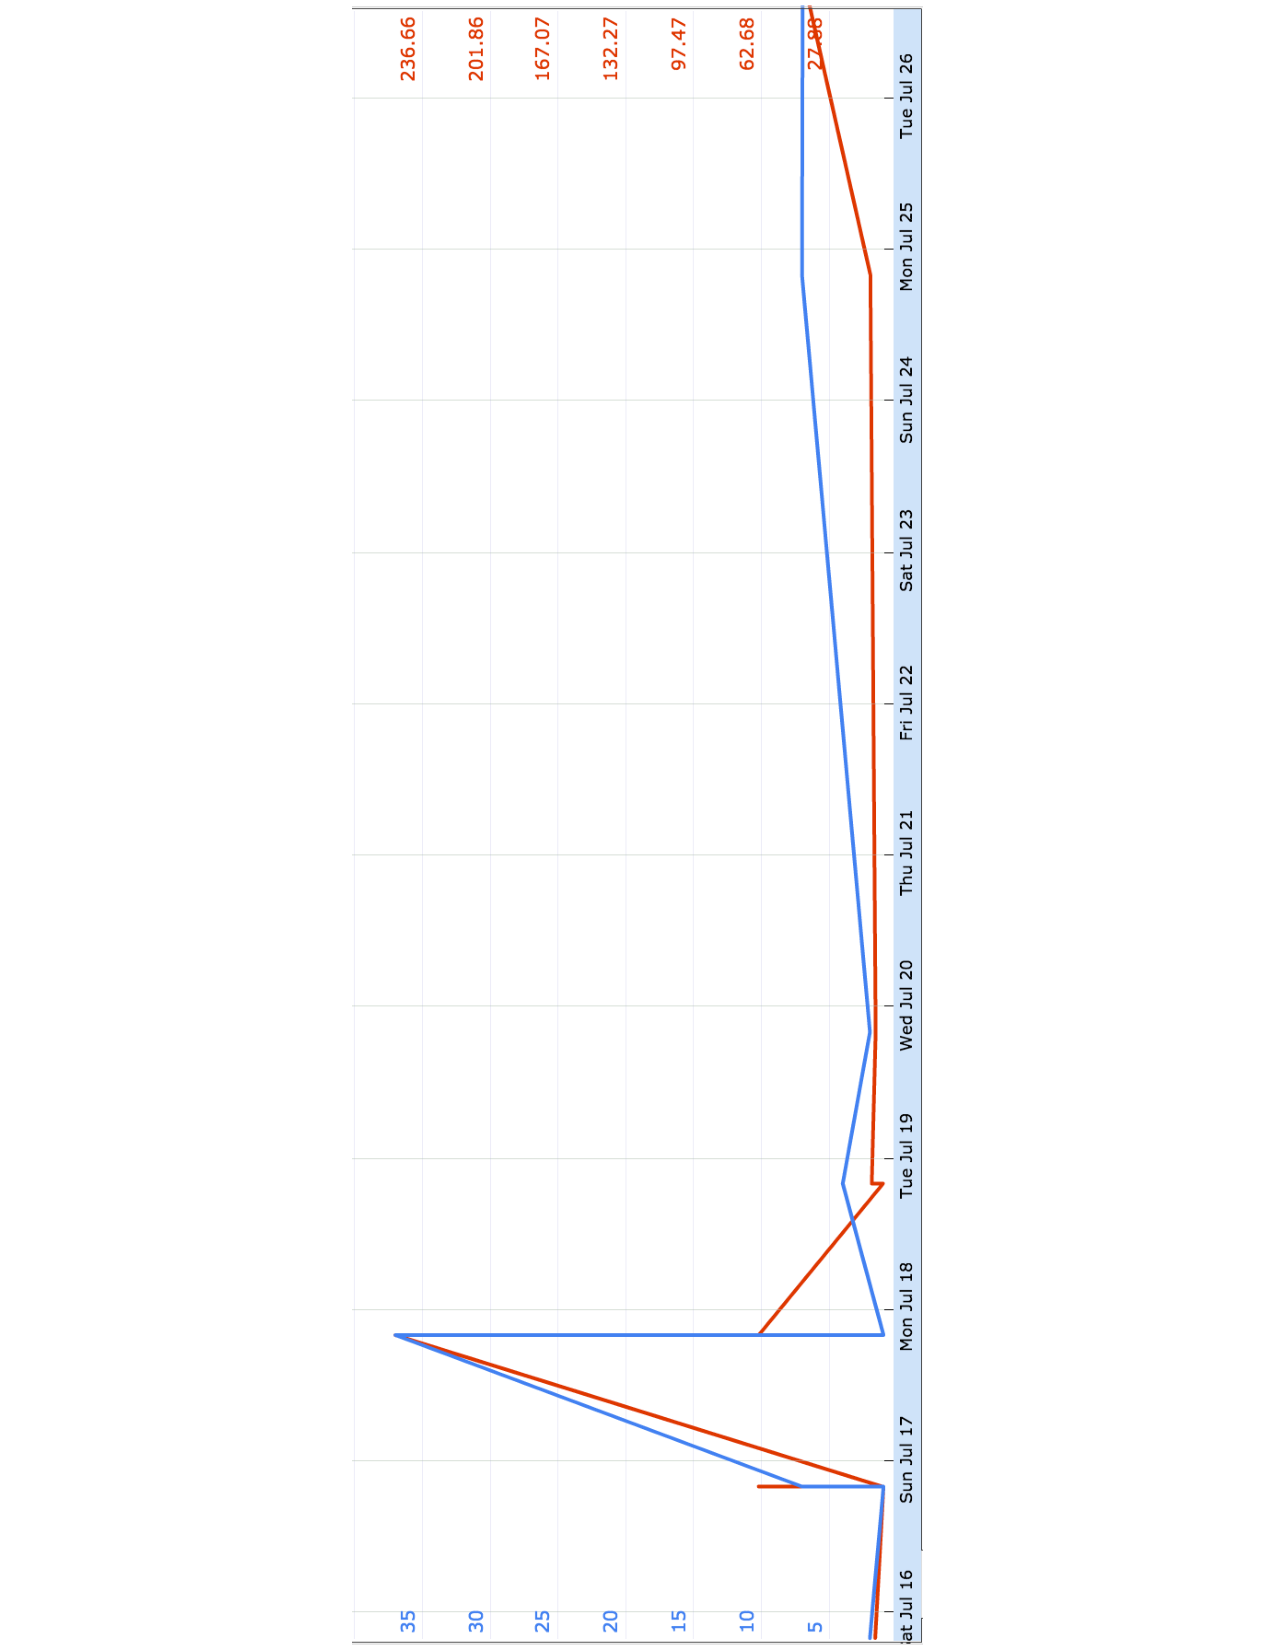
\includegraphics[width=0.49\textwidth]{hack-xsede-usage}
\caption{\footnotesize XSEDE resource utilization for the 10 day period from the start of the Hackathon. The left axis (blue) represents the number of jobs submitted on a daily basis; the right axis (red) represents the number of core-hours utilized. Approximately 1000 total core-hours were used.}
\label{fig:xsede-usage} 
\end{figure}


The majority specifically indicated more hacking time (an extra day or two) would be the most useful addition, with one person suggested scheduling the days so as to not overlap with the co-located event at all.  Given that there were also requests for more pre-event training, we surmise that if domain science participants had been exposed to even just a first level introduction to topics such as using the command line, version control, and job submission, progress would have been considerably accelerated.

On average participants indicated that they had made two new collaborations each and, overall, they felt engaged, empowered, and that the event was well facilitated.  Some of their suggestions for future events included: having some dedicated relevant-package-specific tutors (such as SciDataKit experts) present, more snacks and budget, more pre-event training, and greater input and clarity regarding possible continuation and follow up plans.


\begin{table}[!t]
\centering
\renewcommand{\arraystretch}{1.3}

\caption{*Lines of Code written and commits made from the time of hack repository creation till the end of the hackathon-XSEDE week (22 July 2016).  3 out of 4 repositories have subsequently seen significant contributions beyond this date the data for which have been excluded here.
**As an existing codebase containing thousands of lines of code, the LOC count given here represents the difference in LOC between git repository on 21 July (last day of XSEDE conference after hackathon) and 16 June (day preceding the hackathon)}
\label{stats}
\centering
\begin{tabular}{|c|c|c|p{2cm}|}
\hline
&LOC written* & Commits* & Languages\\
\hline
AerosolDelta & 602 & 70 & Python\\
\hline
SeaIce & 706 & 60 & Python\\
\hline
Parallel OBLIMAP & 80** & 29 & Fortran 90, C, Shell, Make\\
\hline
3DSeals & 284 & 75 & Python\\
\hline
\end{tabular}
\end{table}

Based on the above, what we wish to highlight to the community in this paper, is the potential for using a hackathon as a training and community building event. That is to say, that while many hackathons aim to produce specific products, we found the format to also be an effective (albeit incomplete) means of overcoming some of the challenges discussed in bridging gaps between the HPDC and polar science communities. Clearly, however, pre-event training, trust building, data preparation, and a more appropriate location or co-location event are key issues to be addressed. 

\section{Conclusions and Future Work}
In summary, nowhere is climate change more dramatic than in the polar regions. Studying these regions involves the interactions between an array of specialized domain processes, and multiple heterogeneous data sets that have never been larger. The domain therefore requires HPDC scale resources and yet the broader polar community is largely not currently able to fully utilize them. Prior community engagement and experience have led us to conclude that this is due to a required skills barrier to entry and lack of awareness of available resources. There are other communities addressing the latter, while we have been tasked with addressing the former via our Research Coordination Network.

We have determined that the skills barrier in the polar community is due to: (i) the rate of change in HPDC technologies causing a training lag, (ii) the momentum that exists behind the use of any established methodology, (iii) a lack of domain appropriate training materials, (iv) the fact that polar scientists have an even more restricted time budget for such training than other communities due to required remote field work, and (v) insufficient HPDC support staff on campuses.

While the community is aware of the gap and the broader challenge of equipping interdisciplinary domain scientists - efforts have thus far missed this particular niche.  And while efforts such as SWC are successfully addressing the need for introductions to scientific programming, they fall short of teaching the skills needed for HPDC work. Therefore, in our first attempt to address this gap between the polar community and HPDC use, we used the hackathon model to bring HPDC experts and polar scientists together in a face-to-face and interactive environment.  This enabled a focused period for skills and knowledge exchanges to take place - in both directions - through practical hands on work, using the problems most relevant to the particular domain scientists.  

As a RCN we learnt many valuable lessons about the communities we are trying to bridge. Particularly, the community interaction afforded by organizing and running the hackathon clarified the reasons behind the divide, and the hackathon itself was shown to be an effective means of overcoming some but not all of these challenges.  We have concluded, and intend to test in the future, that the use of a short, intense SWC-like introduction to scientific computing remains necessary to maximize the impact of the hackathon.  

Following this, we would strongly suggest the creation of a HPC-carpentry course that would introduce the further necessary concepts for HPDC work. Specifically, while there are many available resources for HPDC training, unlike prior efforts we suggest that collectively an ALITE-HPDC approach be used.  Such a course would develop HPDC Awareness, Literacy, and following the SWC ethos of teaching only the essentials - be Tailored. That is, it should start with the minimal required basics, be no longer than two days, and crucially involve practical and domain specific examples on HPDC resources. Further, it should be run with and customized for a specific HPDC resource in mind, one that will remain accessible to the users beyond the course duration. That system's specifics (resource requests, job submission, job monitoring, etc.) should be taught so as to equip the users for immediate follow on work, with the goal being to ensure that a user is sufficiently conversant with the domain to move forward. We are currently exploring how both a SWC and an HPC carpentry equivalent might be run within the critical time limits polar science field work demands impose on researchers.  

Based on prior work and literature, such courses would also ideally be followed up on by regular, direct HPDC-expert input over the next 1-2 years. However, where this is not possible given financial or time resource limits - such as field campaigns impose - we propose that a follow up hackathon type event might serve as a quicker alternative mechanism. Such an event is short and moves users beyond simple coursework examples to working on their specific daily science problem on an accessible HPDC resource. Further, the format allows for cross domain networking that can lead to future work and facilitation of work via relationships that would otherwise never have formed.

In our experience, the hackathon model is a valuable means of bridging the divide between science users (such as polar researchers) and HPDC resource operators, tool builders, managers, and funders.  



% use section* for acknowledgement
\section*{Acknowledgement}
This work is supported by NSF ICER 1542110 and associated collaborative
awards. The authors would like to thank the many participants of the Hackathon
and XSEDE'16 Organizing committee for their support.


% trigger a \newpage just before the given reference
% number - used to balance the columns on the last page
% adjust value as needed - may need to be readjusted if
% the document is modified later
\IEEEtriggeratref{9}
% The "triggered" command can be changed if desired:
%\IEEEtriggercmd{\enlargethispage{-5in}}

% references section

% can use a bibliography generated by BibTeX as a .bbl file
% BibTeX documentation can be easily obtained at:
% http://mirror.ctan.org/biblio/bibtex/contrib/doc/
% The IEEEtran BibTeX style support page is at:
% http://www.michaelshell.org/tex/ieeetran/bibtex/
\bibliographystyle{IEEEtran}
% argument is your BibTeX string definitions and bibliography database(s)
\bibliography{./references.bib}
%
% <OR> manually copy in the resultant .bbl file
% set second argument of \begin to the number of references
% (used to reserve space for the reference number labels box)
%\begin{thebibliography}{1}
%
%\bibitem{IEEEhowto:kopka}
%H.~Kopka and P.~W. Daly, \emph{A Guide to \LaTeX}, 3rd~ed.\hskip 1em plus
%  0.5em minus 0.4em\relax Harlow, England: Addison-Wesley, 1999.
%
%\end{thebibliography}
%



% that's all folks
\end{document}


